\section{Problema 2}

\subsection{Enunciado}
En este ejercicio se nos solicita buscar el conjunto dominante mínimo y óptimo dado un grafo cualquiera. Este es un problema del tipo NP completo 
para el cual aún no se encontró forma de resolverlo polinomialmente pero tampoco se demostró que no sea posible solucionarlo con dicha complejidad.

\subsection{Soluci\'on}
Como todavía no se halló algoritmo alguno para resolverlo poliniomalmente y nosotros no somos investigadores/iluminados (aún) decidimos resolverlo
de manera exponencial. Para esto utilizamos el popular método (dicho en criollo) de quedarme con la mejor opción entre poner y no un nodo en el 
conjunto dominante. Este procedimiento lo que hace, básicamente, es analizar todas las soluciones posibles y agarrar la mejor de ellas. \\
%No nos pareció primordial agregarle memorization ya que su complejidad no mejoriría de forma considerable y tampoco nos pareció imperante 
%preocuparnos por la complejidad de la función que chequea si el conjunto recibido es dominante, ya que, mientras sea polinimal, va ser despreciable 
%al lado de la complejidad de analizar todas las soluciones (que como dijimos es exponencial).

\subsection{Pseudocódigo}

global grafoOriginal

\begin{codebox}
\Procname{$\proc{obtenerConjuntoDominanteMinimo}$ (\textbf{in} $Grafo$)}{conjuntoDom}{Conj}
\li	c = crearConj()
\li	grafoOriginal = Grafo
\li	return buscarMinimo(Grafo,c)
\end{codebox}

\begin{codebox}
\Procname{$\proc{buscarMinimo}$(\textbf{in} $Grafo$, \textbf{in} $conjuntoDom$)}{conjuntoDom}{Conj}
\li\textbf{Si} esDominante(conjuntoDom) \textbf{Hacer:} \Do
\li		return conjuntoDom 
\End
\li	\textbf{Si no}  \Do
\li		vertice = grafo.obtenerVertice(); 
\li		grafo = grafo.sinUno()
\li		return min(buscarMinimo(grafo, conjuntoDom), buscarMinimo(grafo, conjuntoDom + vertice)
\li	
\End

\end{codebox}

\begin{codebox}
\Procname{$\proc{esDominante}$(\textbf{in} $Grafo$, \textbf{in} $conjuntoDom$)}{esDominante}{Boolean}
\li \textbf{Para} cada v en V(grafoOriginal) \Do
\li \textbf{Si} conjuntoDom.esta?(v) \textbf{Hacer:} \Do
\li			continue 
		\End
\li \textbf{Si no}  \Do
\li			encontre = false
\li \textbf{Para} cada ver en conjuntoDOm \Do
\li	\textbf{Si} ver.adyacentes.esta?(v) \textbf{Hacer:} \Do	
\li			break
			\End
\li	\textbf{Si} !encontre \textbf{Hacer:} \Do				
\li		return false
			\End
		\End
	\End
\End
	return true
\end{codebox}

La complejidad de mi algoritmo es de $2^n$ * $n^3$. Voy a demostrarlo por inducción:\\

Caso Base:\\

n = 1, si n tiene un solo nodo ver si es dominante me cuesta O(1) ya que recorrer los vertices del grafo original es una sola iteracion y no es posible recorrer sus aristas. Luego divido en el caso en el que uso a ese nodo en el conjunto dominante y el caso en que no. El caso en que no al no tener mas nodos con cual probar me va a devolver el grafo original y el otro caso también ya que el grafo original era el que contenía únicamente a ese nodo. Ambos casos ver si el conjunto es dominante cuesta O(1) ya que tiene a lo sumo una iteración para hacer. Por lo tanto el algoritmo costaría O(1) que es igual a O($2^1*1^3$).\\

Hipótesis inductiva:\\

Supongo que con n nodos la complejidad es $2^n$ * $n^3$\\

Paso inductivo:\\

Quiero ver que con n+1 nodos la complejidad pertenece a $2^{n+1}*(n+1)^3$\\

Ver si el conjunto vacío es dominante me cuesta O(1) ya que en la primera iteración del grafoOriginal no es posible encontrar ningún vertice en el conjunto dominante o adyacente a él. Luego obtengo un nodo del grafo (grafo en el que me guarde todos los vertices, no el origianl) y busco el minimo conjunto dominante agregando ese nodo al conjunto o no, esto por hipótesis inductiva me cuesta 2 * ($2^n * n^3$), ya que tengo que calcular 2 veces el conjunto minimo para n nodos. Por lo tanto la complejidad me termina costando  $2^{n+1}*n^3$ y esto pertence a $2^{n+1}*(n+1)^3$. Con lo cual queda demostrada la complejidad.\\

Notar que esta complejidad esta por encima de la complejidad exacta, ya que el $n^3$ variaría en cada iteración dependiendo de la cantidad de nodos en el conjuntoDominante.

\subsection{Peor Caso}

Como el algoritmo es exacto y recorre todas las soluciones posibles siempre obtiene la mejor de ellas. Por lo tanto no existe una 'peor' instancia
en la que la solución devuelta sea sub-óptima, siempre devuelve la mejor.

\subsection{Tests y análisis}
En los siguientes gráfico podemos observar que la cantidad de ciclos y el tiempo crecen notablemente a medida que el grafo tiene cada vez mas nodos.\\
Esto es debido a que, como dijimos anteriormente, la complejidad es exponencial en el tamaño de la entrada (en este caso, la cantidad de nodos 
del grafo) y no existe un mejor o peor en caso en el cual la complejidad sea mucho menor a O($2^n*n^3$). Por esto es que tanto en el grafico de tiempos
 como en el de ciclos se puede observar claramente que la complejidad es exponencial.

\begin {center}
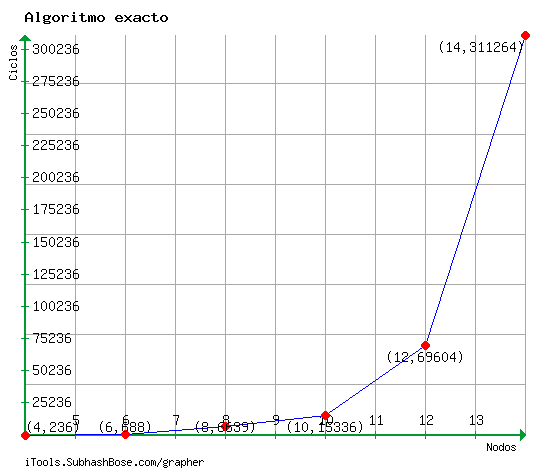
\includegraphics[width=12cm]{./graficos/exacto.png}
% grafico.eps: 0x0 pixel, 300dpi, 0.00x0.00 cm, bb=50 50 410 302
\end {center} 

\begin {center}
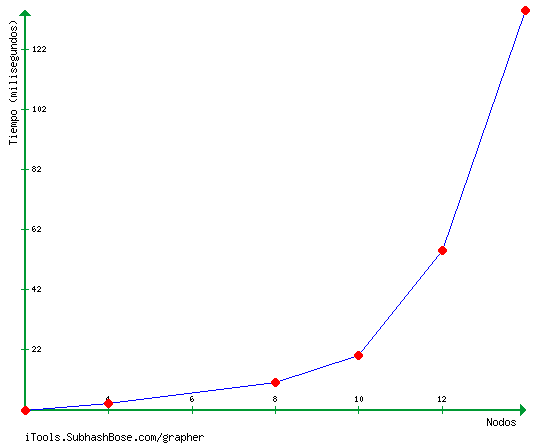
\includegraphics[width=12cm]{./graficos/exactoConTiempo.png}
% grafico.eps: 0x0 pixel, 300dpi, 0.00x0.00 cm, bb=50 50 410 302
\end {center}
